\documentclass{extbook}[14pt]
\usepackage{multicol, enumerate, enumitem, hyperref, color, soul, setspace, parskip, fancyhdr, amssymb, amsthm, amsmath, bbm, latexsym, units, mathtools}
\everymath{\displaystyle}
\usepackage[headsep=0.5cm,headheight=0cm, left=1 in,right= 1 in,top= 1 in,bottom= 1 in]{geometry}
\usepackage{dashrule}  % Package to use the command below to create lines between items
\newcommand{\litem}[1]{\item #1

\rule{\textwidth}{0.4pt}}
\pagestyle{fancy}
\lhead{}
\chead{Answer Key for Progress Quiz 4 Version C}
\rhead{}
\lfoot{9187-5854}
\cfoot{}
\rfoot{Spring 2021}
\begin{document}
\textbf{This key should allow you to understand why you choose the option you did (beyond just getting a question right or wrong). \href{https://xronos.clas.ufl.edu/mac1105spring2020/courseDescriptionAndMisc/Exams/LearningFromResults}{More instructions on how to use this key can be found here}.}

\textbf{If you have a suggestion to make the keys better, \href{https://forms.gle/CZkbZmPbC9XALEE88}{please fill out the short survey here}.}

\textit{Note: This key is auto-generated and may contain issues and/or errors. The keys are reviewed after each exam to ensure grading is done accurately. If there are issues (like duplicate options), they are noted in the offline gradebook. The keys are a work-in-progress to give students as many resources to improve as possible.}

\rule{\textwidth}{0.4pt}

\begin{enumerate}\litem{
Which of the following equations \textit{could} be of the graph presented below?

\begin{center}
    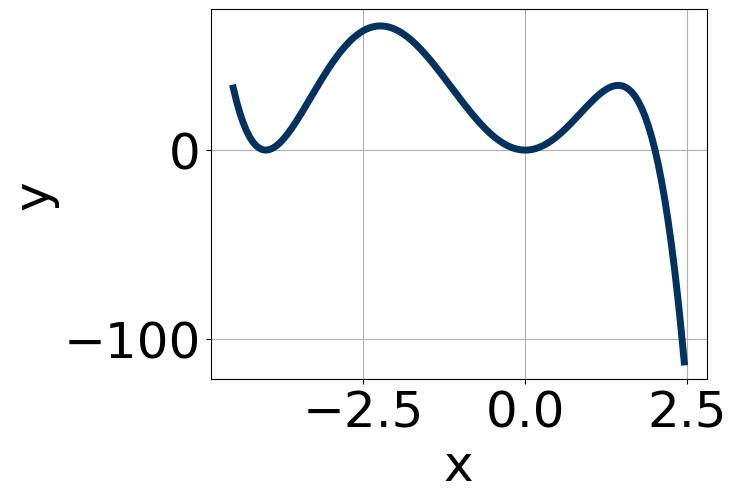
\includegraphics[width=0.5\textwidth]{../Figures/polyGraphToFunctionCopyC.png}
\end{center}


The solution is \( -8(x - 3)^{4} (x - 1)^{5} (x + 3)^{7} \), which is option C.\begin{enumerate}[label=\Alph*.]
\item \( -18(x - 3)^{4} (x - 1)^{6} (x + 3)^{9} \)

The factor $(x - 1)$ should have an odd power.
\item \( 13(x - 3)^{8} (x - 1)^{9} (x + 3)^{6} \)

The factor $(x + 3)$ should have an odd power and the leading coefficient should be the opposite sign.
\item \( -8(x - 3)^{4} (x - 1)^{5} (x + 3)^{7} \)

* This is the correct option.
\item \( 10(x - 3)^{6} (x - 1)^{9} (x + 3)^{11} \)

This corresponds to the leading coefficient being the opposite value than it should be.
\item \( -19(x - 3)^{5} (x - 1)^{10} (x + 3)^{5} \)

The factor $3$ should have an even power and the factor $1$ should have an odd power.
\end{enumerate}

\textbf{General Comment:} General Comments: Draw the x-axis to determine which zeros are touching (and so have even multiplicity) or cross (and have odd multiplicity).
}
\litem{
Describe the end behavior of the polynomial below.
\[ f(x) = -3(x - 3)^{5}(x + 3)^{6}(x - 2)^{3}(x + 2)^{5} \]The solution is the graph below, which is option A.
\begin{center}
    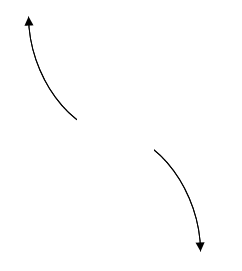
\includegraphics[width=0.3\textwidth]{../Figures/polyEndBehaviorCopyAC.png}
\end{center}\begin{enumerate}[label=\Alph*.]
\begin{multicols}{2}
\item 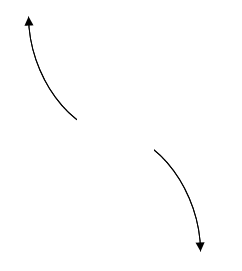
\includegraphics[width = 0.3\textwidth]{../Figures/polyEndBehaviorCopyAC.png}
\item 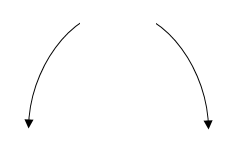
\includegraphics[width = 0.3\textwidth]{../Figures/polyEndBehaviorCopyBC.png}
\item 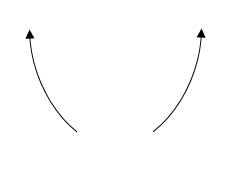
\includegraphics[width = 0.3\textwidth]{../Figures/polyEndBehaviorCopyCC.png}
\item 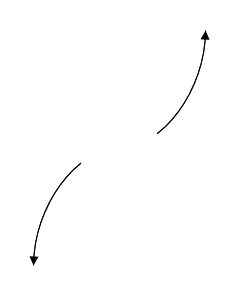
\includegraphics[width = 0.3\textwidth]{../Figures/polyEndBehaviorCopyDC.png}
\end{multicols}\item None of the above.\end{enumerate}
\textbf{General Comment:} Remember that end behavior is determined by the leading coefficient AND whether the \textbf{sum} of the multiplicities is positive or negative.
}
\litem{
Construct the lowest-degree polynomial given the zeros below. Then, choose the intervals that contain the coefficients of the polynomial in the form $ax^3+bx^2+cx+d$.
\[ 4, -7, \text{ and } \frac{-1}{5} \]The solution is \( 5x^{3} +16 x^{2} -137 x -28 \), which is option C.\begin{enumerate}[label=\Alph*.]
\item \( a \in [4, 10], b \in [53.5, 57.4], c \in [150, 154], \text{ and } d \in [23, 37] \)

$5x^{3} +56 x^{2} +151 x + 28$, which corresponds to multiplying out $(x + 4)(x + 7)(5x + 1)$.
\item \( a \in [4, 10], b \in [14.4, 17.4], c \in [-139, -134], \text{ and } d \in [23, 37] \)

$5x^{3} +16 x^{2} -137 x + 28$, which corresponds to multiplying everything correctly except the constant term.
\item \( a \in [4, 10], b \in [14.4, 17.4], c \in [-139, -134], \text{ and } d \in [-35, -21] \)

* $5x^{3} +16 x^{2} -137 x -28$, which is the correct option.
\item \( a \in [4, 10], b \in [-17.7, -14.1], c \in [-139, -134], \text{ and } d \in [23, 37] \)

$5x^{3} -16 x^{2} -137 x + 28$, which corresponds to multiplying out $(x + 4)(x -7)(5x -1)$.
\item \( a \in [4, 10], b \in [-14.4, -12.2], c \in [-147, -141], \text{ and } d \in [-35, -21] \)

$5x^{3} -14 x^{2} -143 x -28$, which corresponds to multiplying out $(x + 4)(x -7)(5x + 1)$.
\end{enumerate}

\textbf{General Comment:} To construct the lowest-degree polynomial, you want to multiply out $(x -4)(x + 7)(5x + 1)$
}
\litem{
Describe the zero behavior of the zero $x = 9$ of the polynomial below.
\[ f(x) = 2(x - 8)^{12}(x + 8)^{8}(x + 9)^{7}(x - 9)^{4} \]The solution is the graph below, which is option C.
\begin{center}
    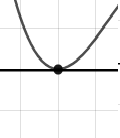
\includegraphics[width=0.3\textwidth]{../Figures/polyZeroBehaviorCC.png}
\end{center}\begin{enumerate}[label=\Alph*.]
\begin{multicols}{2}
\item 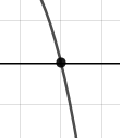
\includegraphics[width = 0.3\textwidth]{../Figures/polyZeroBehaviorAC.png}
\item 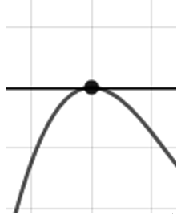
\includegraphics[width = 0.3\textwidth]{../Figures/polyZeroBehaviorBC.png}
\item 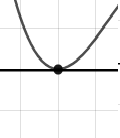
\includegraphics[width = 0.3\textwidth]{../Figures/polyZeroBehaviorCC.png}
\item 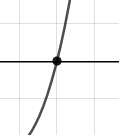
\includegraphics[width = 0.3\textwidth]{../Figures/polyZeroBehaviorDC.png}
\end{multicols}\item None of the above.\end{enumerate}
\textbf{General Comment:} You will need to sketch the entire graph, then zoom in on the zero the question asks about.
}
\litem{
Describe the end behavior of the polynomial below.
\[ f(x) = 8(x + 8)^{2}(x - 8)^{3}(x + 7)^{5}(x - 7)^{7} \]The solution is the graph below, which is option D.
\begin{center}
    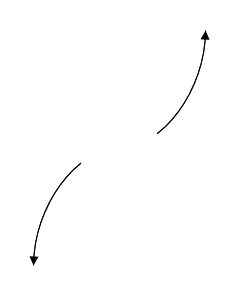
\includegraphics[width=0.3\textwidth]{../Figures/polyEndBehaviorDC.png}
\end{center}\begin{enumerate}[label=\Alph*.]
\begin{multicols}{2}
\item 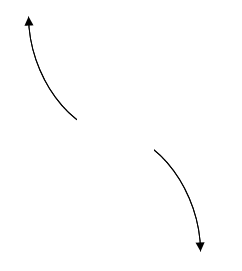
\includegraphics[width = 0.3\textwidth]{../Figures/polyEndBehaviorAC.png}
\item 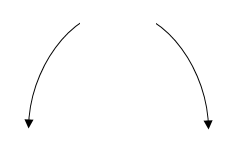
\includegraphics[width = 0.3\textwidth]{../Figures/polyEndBehaviorBC.png}
\item 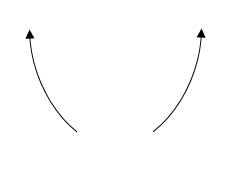
\includegraphics[width = 0.3\textwidth]{../Figures/polyEndBehaviorCC.png}
\item 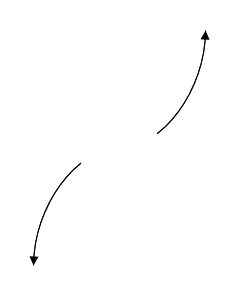
\includegraphics[width = 0.3\textwidth]{../Figures/polyEndBehaviorDC.png}
\end{multicols}\item None of the above.\end{enumerate}
\textbf{General Comment:} Remember that end behavior is determined by the leading coefficient AND whether the \textbf{sum} of the multiplicities is positive or negative.
}
\litem{
Construct the lowest-degree polynomial given the zeros below. Then, choose the intervals that contain the coefficients of the polynomial in the form $x^3+bx^2+cx+d$.
\[ 2 - 5 i \text{ and } -1 \]The solution is \( x^{3} -3 x^{2} +25 x + 29 \), which is option C.\begin{enumerate}[label=\Alph*.]
\item \( b \in [-1.3, 1.7], c \in [5, 12], \text{ and } d \in [4, 6] \)

$x^{3} + x^{2} +6 x + 5$, which corresponds to multiplying out $(x + 5)(x + 1)$.
\item \( b \in [-1.3, 1.7], c \in [-5, 2], \text{ and } d \in [-4, 0] \)

$x^{3} + x^{2} -x -2$, which corresponds to multiplying out $(x -2)(x + 1)$.
\item \( b \in [-5.6, -2.4], c \in [25, 27], \text{ and } d \in [24, 31] \)

* $x^{3} -3 x^{2} +25 x + 29$, which is the correct option.
\item \( b \in [2.7, 5.9], c \in [25, 27], \text{ and } d \in [-35, -24] \)

$x^{3} +3 x^{2} +25 x -29$, which corresponds to multiplying out $(x-(2 - 5 i))(x-(2 + 5 i))(x -1)$.
\item \( \text{None of the above.} \)

This corresponds to making an unanticipated error or not understanding how to use nonreal complex numbers to create the lowest-degree polynomial. If you chose this and are not sure what you did wrong, please contact the coordinator for help.
\end{enumerate}

\textbf{General Comment:} Remember that the conjugate of $a+bi$ is $a-bi$. Since these zeros always come in pairs, we need to multiply out $(x-(2 - 5 i))(x-(2 + 5 i))(x-(-1))$.
}
\litem{
Which of the following equations \textit{could} be of the graph presented below?

\begin{center}
    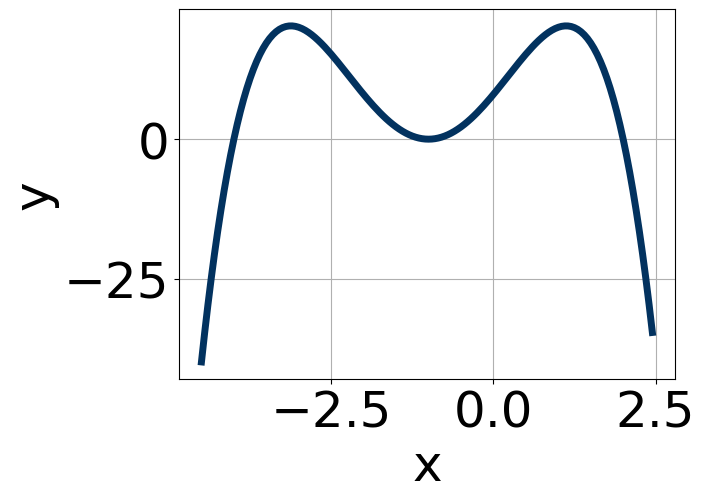
\includegraphics[width=0.5\textwidth]{../Figures/polyGraphToFunctionC.png}
\end{center}


The solution is \( -11x^{4} (x - 3)^{10} (x + 2)^{6} \), which is option B.\begin{enumerate}[label=\Alph*.]
\item \( 20x^{8} (x - 3)^{10} (x + 2)^{4} \)

This corresponds to the leading coefficient being the opposite value than it should be.
\item \( -11x^{4} (x - 3)^{10} (x + 2)^{6} \)

* This is the correct option.
\item \( -15x^{10} (x - 3)^{6} (x + 2)^{9} \)

The factor $(x + 2)$ should have an even power.
\item \( -2x^{6} (x - 3)^{5} (x + 2)^{11} \)

The factors $(x - 3)$ and $(x + 2)$ should both have even powers.
\item \( 17x^{4} (x - 3)^{8} (x + 2)^{7} \)

The factor $(x + 2)$ should have an even power and the leading coefficient should be the opposite sign.
\end{enumerate}

\textbf{General Comment:} General Comments: Draw the x-axis to determine which zeros are touching (and so have even multiplicity) or cross (and have odd multiplicity).
}
\litem{
Construct the lowest-degree polynomial given the zeros below. Then, choose the intervals that contain the coefficients of the polynomial in the form $x^3+bx^2+cx+d$.
\[ -4 + 3 i \text{ and } 2 \]The solution is \( x^{3} +6 x^{2} +9 x -50 \), which is option A.\begin{enumerate}[label=\Alph*.]
\item \( b \in [2, 11], c \in [8, 12], \text{ and } d \in [-53, -49] \)

* $x^{3} +6 x^{2} +9 x -50$, which is the correct option.
\item \( b \in [-2, 4], c \in [-1, 3], \text{ and } d \in [-10, -6] \)

$x^{3} + x^{2} +2 x -8$, which corresponds to multiplying out $(x + 4)(x -2)$.
\item \( b \in [-2, 4], c \in [-5, -3], \text{ and } d \in [6, 8] \)

$x^{3} + x^{2} -5 x + 6$, which corresponds to multiplying out $(x -3)(x -2)$.
\item \( b \in [-10, -5], c \in [8, 12], \text{ and } d \in [46, 54] \)

$x^{3} -6 x^{2} +9 x + 50$, which corresponds to multiplying out $(x-(-4 + 3 i))(x-(-4 - 3 i))(x + 2)$.
\item \( \text{None of the above.} \)

This corresponds to making an unanticipated error or not understanding how to use nonreal complex numbers to create the lowest-degree polynomial. If you chose this and are not sure what you did wrong, please contact the coordinator for help.
\end{enumerate}

\textbf{General Comment:} Remember that the conjugate of $a+bi$ is $a-bi$. Since these zeros always come in pairs, we need to multiply out $(x-(-4 + 3 i))(x-(-4 - 3 i))(x-(2))$.
}
\litem{
Describe the zero behavior of the zero $x = 5$ of the polynomial below.
\[ f(x) = 5(x + 5)^{7}(x - 5)^{10}(x + 3)^{5}(x - 3)^{6} \]The solution is the graph below, which is option C.
\begin{center}
    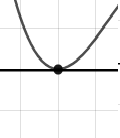
\includegraphics[width=0.3\textwidth]{../Figures/polyZeroBehaviorCopyCC.png}
\end{center}\begin{enumerate}[label=\Alph*.]
\begin{multicols}{2}
\item 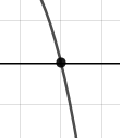
\includegraphics[width = 0.3\textwidth]{../Figures/polyZeroBehaviorCopyAC.png}
\item 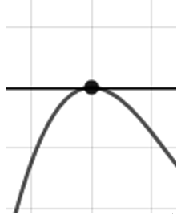
\includegraphics[width = 0.3\textwidth]{../Figures/polyZeroBehaviorCopyBC.png}
\item 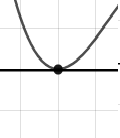
\includegraphics[width = 0.3\textwidth]{../Figures/polyZeroBehaviorCopyCC.png}
\item 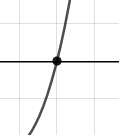
\includegraphics[width = 0.3\textwidth]{../Figures/polyZeroBehaviorCopyDC.png}
\end{multicols}\item None of the above.\end{enumerate}
\textbf{General Comment:} You will need to sketch the entire graph, then zoom in on the zero the question asks about.
}
\litem{
Construct the lowest-degree polynomial given the zeros below. Then, choose the intervals that contain the coefficients of the polynomial in the form $ax^3+bx^2+cx+d$.
\[ 3, 6, \text{ and } \frac{-4}{3} \]The solution is \( 3x^{3} -23 x^{2} +18 x + 72 \), which is option A.\begin{enumerate}[label=\Alph*.]
\item \( a \in [2, 12], b \in [-24, -18], c \in [16, 19], \text{ and } d \in [72, 73] \)

* $3x^{3} -23 x^{2} +18 x + 72$, which is the correct option.
\item \( a \in [2, 12], b \in [-24, -18], c \in [16, 19], \text{ and } d \in [-77, -68] \)

$3x^{3} -23 x^{2} +18 x -72$, which corresponds to multiplying everything correctly except the constant term.
\item \( a \in [2, 12], b \in [20, 24], c \in [16, 19], \text{ and } d \in [-77, -68] \)

$3x^{3} +23 x^{2} +18 x -72$, which corresponds to multiplying out $(x + 3)(x + 6)(3x -4)$.
\item \( a \in [2, 12], b \in [-12, -2], c \in [-67, -60], \text{ and } d \in [-77, -68] \)

$3x^{3} -5 x^{2} -66 x -72$, which corresponds to multiplying out $(x + 3)(x -6)(3x + 4)$.
\item \( a \in [2, 12], b \in [27, 34], c \in [90, 95], \text{ and } d \in [72, 73] \)

$3x^{3} +31 x^{2} +90 x + 72$, which corresponds to multiplying out $(x + 3)(x + 6)(3x + 4)$.
\end{enumerate}

\textbf{General Comment:} To construct the lowest-degree polynomial, you want to multiply out $(x -3)(x -6)(3x + 4)$
}
\end{enumerate}

\end{document}